
\section{Theorie}
\label{sec:Theorie}

\subsection{Fresnelsche und Fraunhofersche Lichtbeugung}

Trifft Licht auf eine Öffnung, deren Abmessungen in der Größenordnung der Wellenlänge des Lichtes entsprechen, so tritt Beugung auf und es kann in der Beobachtungsebene eine Beugungsfigur beobachtet werden, welche die Intensität $I$ des Lichtes in Abhängigkeit des Beugungswinkels $\phi$ beschreibt. 
Wird das Licht als Welle aufgefasst, so kann dieser Effekt mit dem Huygensschen Prinzip erklärt werden. Dieses besagt, dass jeder Punkt der Wellenfront der Ursprung einer neuen kugelförmigen Elementarwelle ist, deren Einhüllende die neue Wellenfront ergibt.\\
Dabei wird im wesentlichen zwischen zwei verschiedenen Beugungsarten unterschieden, der Fresnelschen  und der Fraunhoferschen Lichtbeugung (Abbildung \ref{fig:FFB}). Die Fresnelsche Beugung tritt auf, wenn die Lichtquelle und der Beobachtungspunkt in Bezug auf die Öffnungsgröße nahe an der Öffnung sind, sodass divergente Strahlenbündel auftreten. An einem Punkt $P$ in der Beobachtungsebene interferieren somit Strahlen, die unter verschiedenen Winkeln $\phi_i$ gebeugt werden. Bei der Fraunhoferschen Beugung sind Lichtquelle und Beobachtungspunkt im Vergleich zur Öffnungsgröße nahezu unendlich weit von der Öffnung entfernt, sodass von einem parallel einfallendem Lichtbündel ausgegangen werden kann. Alle Strahlen, die hier an einem Punkt $P$ in der Beobachtungsebene interferieren, werden nahezu unter dem selben Winkel $\phi$ gebeugt. Das parallel einfallende Licht kann ebenfalls durch einen Laser und der große Abstand der Beobachtungsebene zur Öffnung durch eine Sammellinse realisiert werden. Im folgenden wird immer von der Fraunhoferschen Lichtbeugung ausgegangen.

\begin{figure}
	\centering
	\caption{Fresnelsche und Fraunhofersche Lichtbeugung am Einzelspalt \cite{V406}.}
	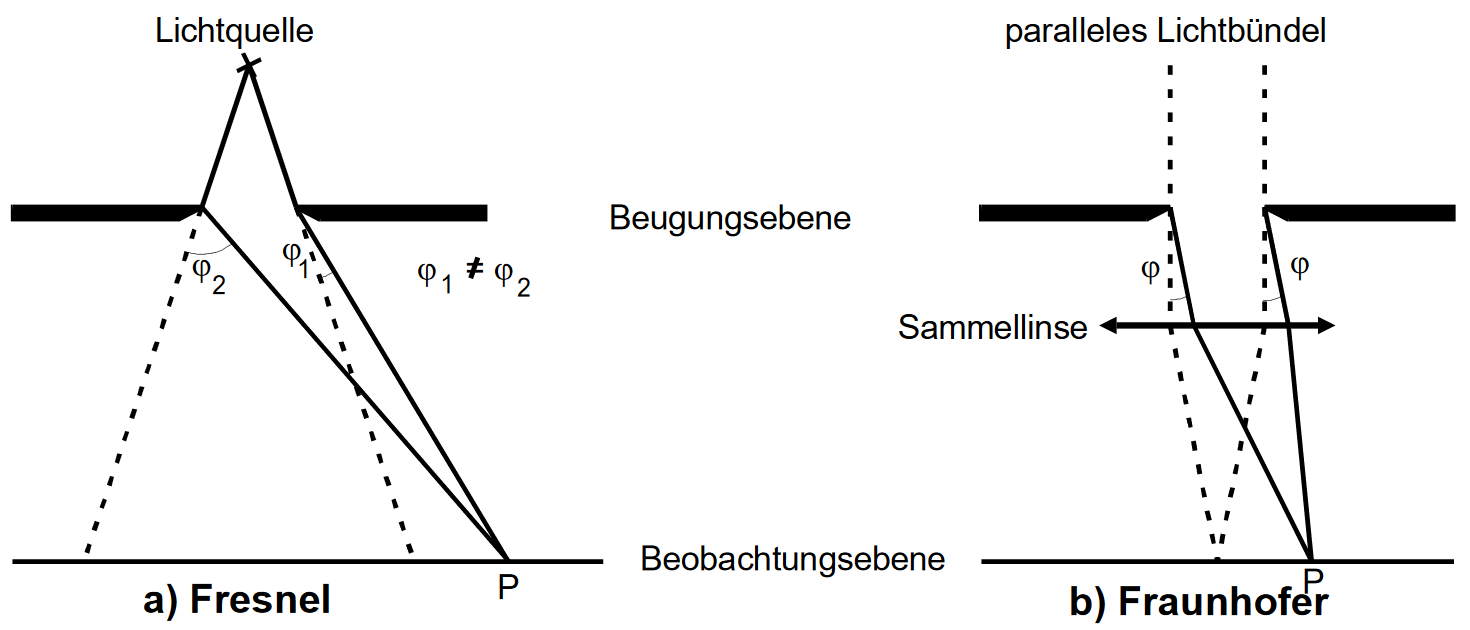
\includegraphics[width=\linewidth-70pt,height=\textheight-70pt,keepaspectratio]{content/images/FresnelFrauenhoferBeugung.png}
	\label{fig:FFB}
\end{figure}

\subsection{Lichtbeugung am Einzel- und Doppelspalt}

Es wird nun als Öffnung in der Beugungsebene ein Spalt betrachtet, dessen breite $b$ klein gegenüber seiner Länge ist, sodass das Licht nur in einer Dimension gebeugt wird. 
Um die Amplitude in einem Punkt $P$ der Beobachtungsebene zu bestimmen, muss nach dem Huygensschen Prinzip die Überlagerung sämtlicher Elementarwellen betrachtet werden, die zum selben Zeitpunkt in $P$ ankommen. Es muss also über die gesamte Spaltbreite $b$ integriert werden, wobei aus Abbildung \ref{fig:Einzelspalt} hervorgeht, dass die einzelnen Strahlenbündel eine Phasendifferenz von 
\[
\delta = \frac{2\pi x \sin \phi}{\lambda}
\]
besitzen. Wird von einer sich in $z$-Richtung ausbreiten einfallenden Welle der Form
\[
A(z,t) = A_0\exp \left(i\left(\omega t-\frac{2\pi z}{\lambda}\right)\right)
\]
ausgegangen, ergibt sich für die Amplitude $B$ des in $\phi$-Richtung abgelenkten Strahls:
\[
B(z,t,\phi) = A_0 \int_0^b\exp\left(i\left(\omega t-\frac{2\pi z}{\lambda}+\delta\right)\right).dx\text{.}
\]
Nach ausführen des Integrals und unter Vernachlässigung der für das Experiment irrelevanten Terme ergibt sich mit der Vereinfachung
\[
\eta(x) := \frac{\pi x \sin \phi}{\lambda}
\]
schließlich:
\[
B_1(\phi) = A_0b\frac{\sin \eta(b)}{\eta(b)}\text{.}
\]
Da $B(\phi)$ nicht direkt gemessen werden kann, wird die zeitlich gemittelte Intensität $I(\phi)$ betrachtet :
\begin{equation}
I_1(\phi)\propto B^2_1(\phi) \propto \frac{\sin^2 \eta(b)}{\eta^2(b)}\text{.} \label{eq:I1}
\end{equation}
Bei dem Doppelspalt berechnet sich die Intensität analog, da er als Überlagerung zweier Einzelspalte der Breite $b$ im Abstand $s$ aufgefasst werden kann (vergleiche Abbildung \ref{fig:Doppelspalt}):
\begin{equation}
I_2(\phi) \propto \cos^2\eta(s) I_1(\phi) \propto \cos^2\eta(s)\frac{\sin^2 \eta(b)}{\eta^2(b)}\text{.}\label{eq:I2}
\end{equation}
Es ist zu erkennen, dass zur Intensitätsverteilung des Einzelspalts eine $\cos^2$ Verteilung hinzukommt, welche vom Spaltabstand $s$ abhängt.

\begin{figure}
	\centering
	\caption{Skizze zur Bestimmung der Phasendifferenz am Einzelspalt \cite{V406}.}
	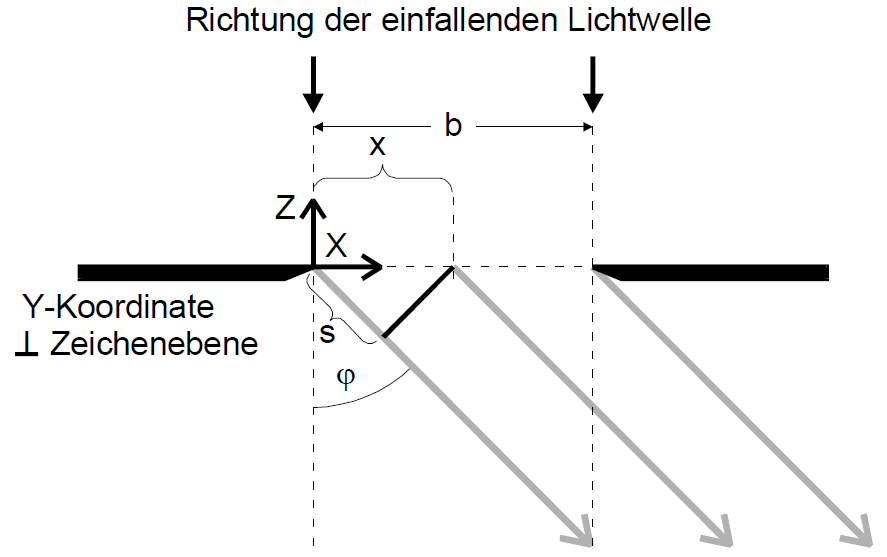
\includegraphics[width=\linewidth-150pt,height=\textheight-150pt,keepaspectratio]{content/images/Einzelspalt.png}
	\label{fig:Einzelspalt}
\end{figure}

\begin{figure}
	\centering
	\caption{Skizze für den Doppelspalt \cite{V406}.}
	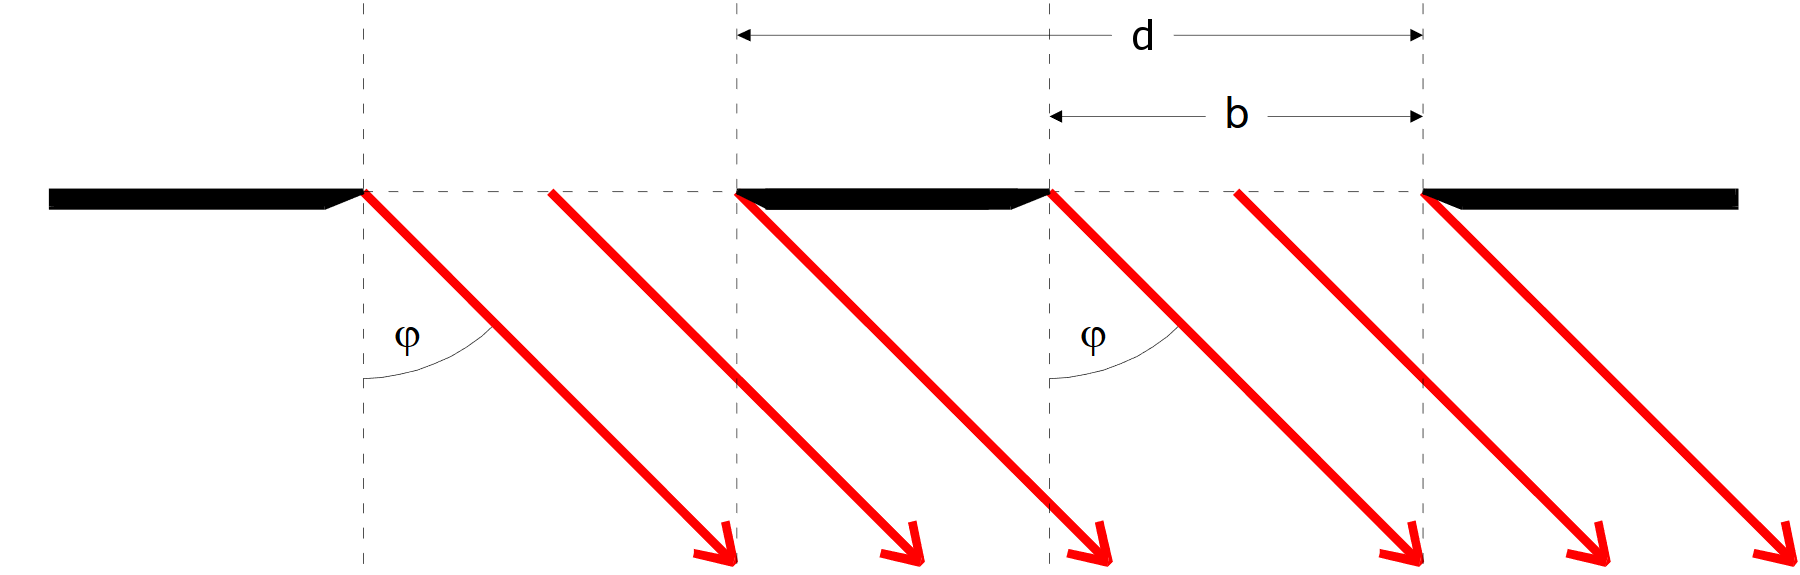
\includegraphics[width=\linewidth-70pt,height=\textheight-70pt,keepaspectratio]{content/images/Doppelspalt.png}
	\label{fig:Doppelspalt}
\end{figure}